\chapter{Arrays and Linked Lists}

We will talk more about arrays and new concepts including linked lists, pointers and time complexity in this chapter.

\section{Arrays in memory}

Let's go back to the example in Chapter 2.

\begin{lstlisting}
int x[] = {3,1,4,1,5,9,2,6};

cout << x[0] << endl; //3 
cout << x[4] << endl; //5
cout << x[7] << endl; //6 (last element)
cout << x[8] << endl; //unexpected value 
\end{lstlisting}

The reason for \texttt{x[8]} to return an unexpected value rather than an error is pretty interesting. To understand that, you will need to know how arrays are stored in memory, and how array elements are accessed. 

A \textbf{continuous} memory is allocated for each array. As indicated in the figure.

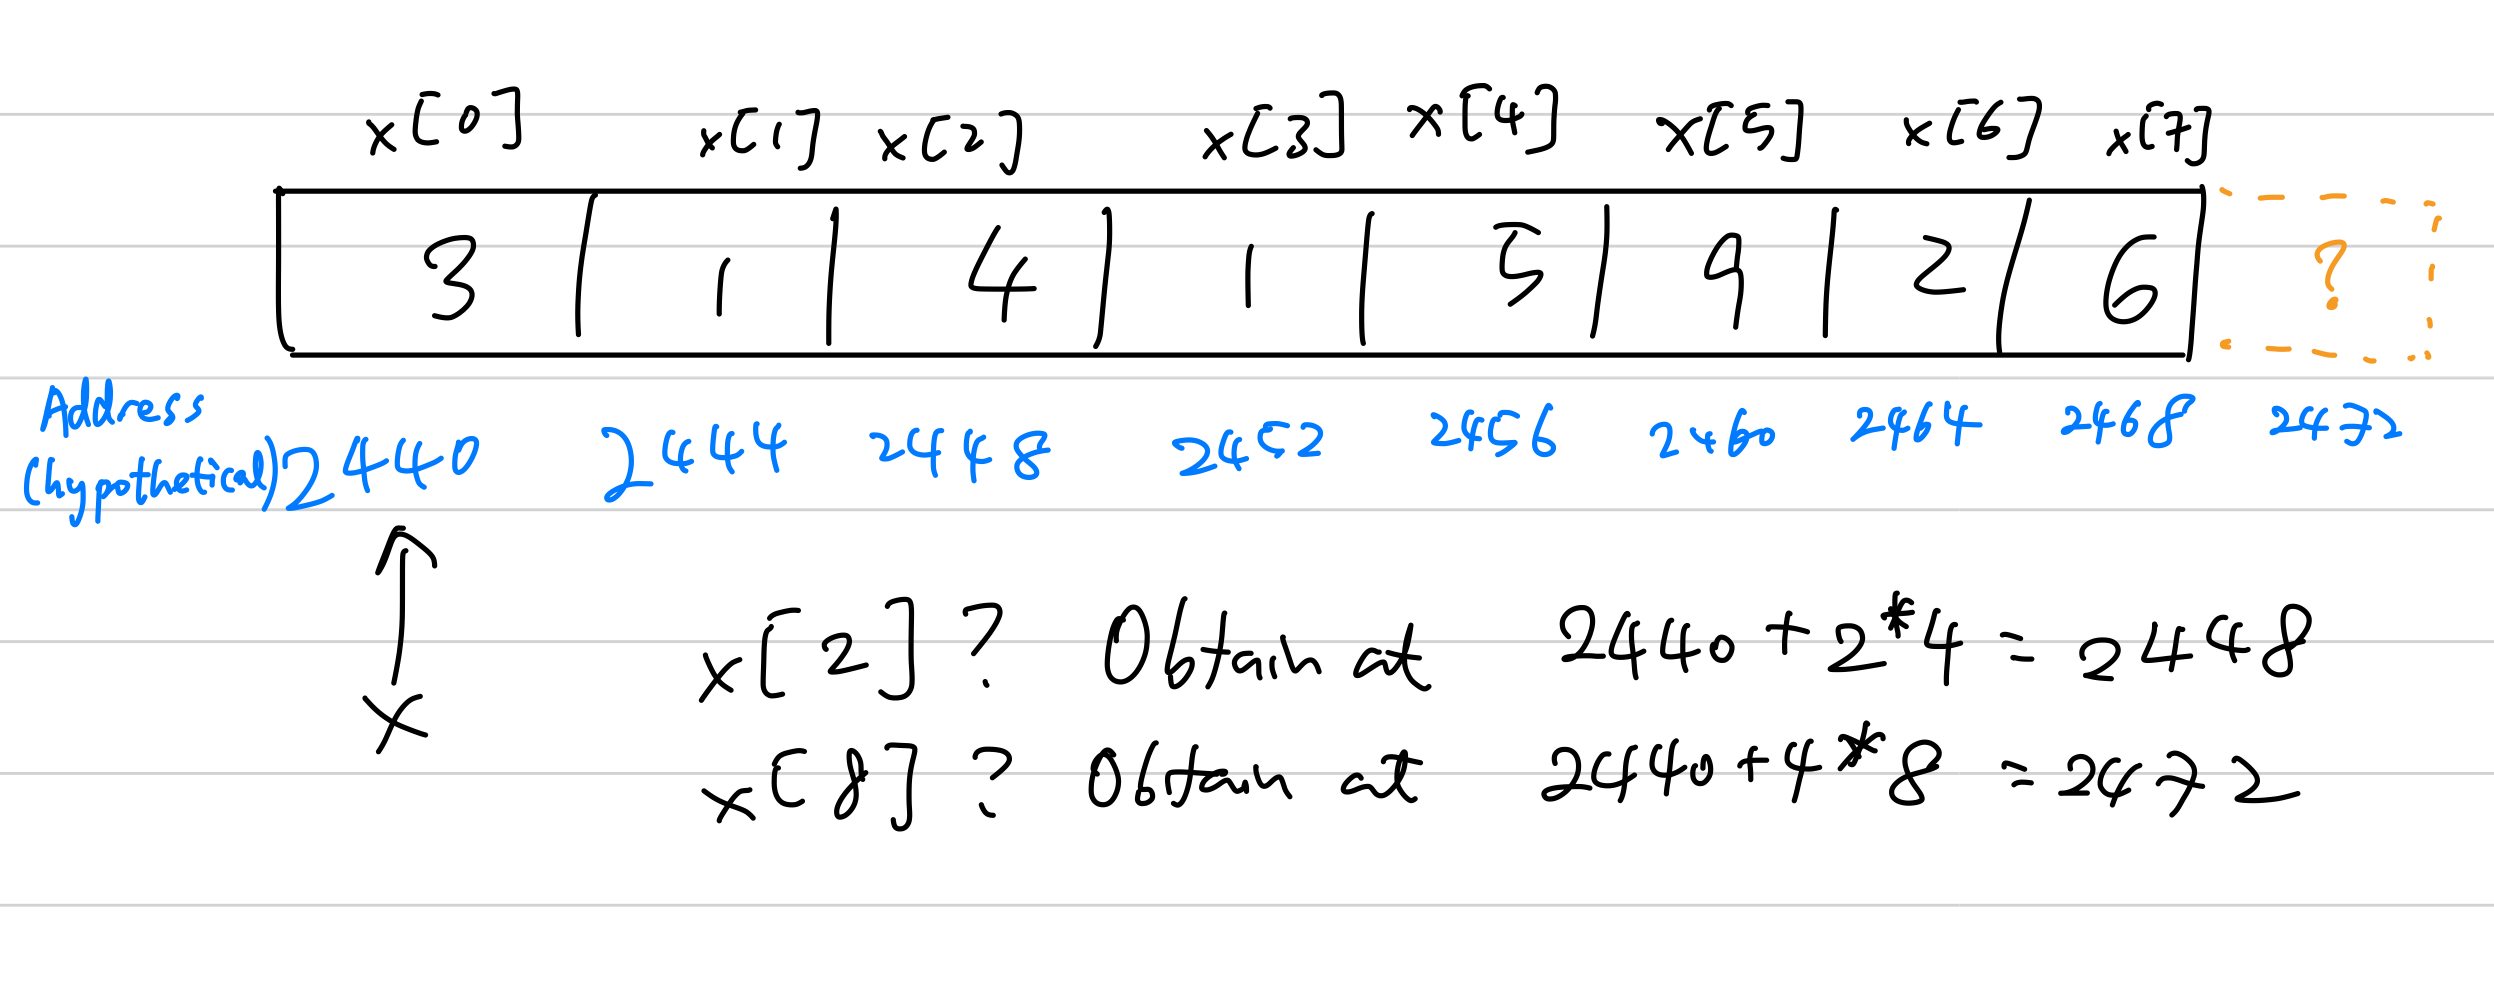
\includegraphics[width=13cm]{ch5-array.png}

C++ stores the \textbf{base address}\index{base address} of the array x, say at location 2240. Then to obtain \texttt{x[k]}, it will calculate the address that it needs to retrieve by $2240 + k*4$, the $*4$ is there because each integer occupies 4 bytes of memory, the multiplier is different depending on different data types. 

For example, when querying \texttt{x[4]}, we obtained it from address $2240+16 = 2256$. 

So, when querying \texttt{x[8]}, we obtained it from address $2240+32 = 2272$. What is in address 2272? We don't know! It is just a bunch of random 0s and 1s last modified by other programs. 
\vspace{6mm}

If you run this program multiple times, the result printed is different, this is because the base address allocated for the array by the program is different every time. 

As the location of \texttt{x[8]} is different, it probably stores a different sequence of 0s and 1s. While x[0..7] are the same, because that is what \texttt{int x[8] = \{3,1,4,1,5,9,2,6\};} does, put 3 at base address, put 1 at base address + 4, put 4 at base address + 8 ..., once the base address is allocated.

\section{Pointers}

\textit{Of less importance, difficult topic}
\vspace{6mm}

Don't have time to cover, there should be plenty of resources online on this topic, including mycodeschool's playlist on pointers.

\section{Pointers and arrays}

\textit{Difficult topic}
\vspace{6mm}

Although we did not cover pointers in depth, it is important to understand the usage of pointers in manipulating arrays. 

First, we need to understand that there are two ways values are passed by a function call, that is, call by reference\index{call by reference} and call by value\index{call by value}, you will need to be able to distinguish when each type is used.

\subsection{Call by value}

Primary data types (those you saw in section 3.1, e.g. \texttt{int}, \texttt{char}, \texttt{float}) are normally called by value, which means that their value is copied when they are passed into another function. Changes made to the variable inside the function will not affect its value in the caller. It is better to demonstrate through an example.

\begin{lstlisting}
void change(int a){ //pass by value
    a += 1;
    cout << "In change: " << a << endl; //In change: 6
    return;
}
int main(){
    int a = 5;
    change(a);
    cout << "In main: " << a << endl; //In main: 5
}
\end{lstlisting}

As you can see, although \texttt{a} is changed to 6 in the change function, it is still 5 in the main function. 
\vspace{6mm}

If you would like to actually change the value of \texttt{a}, you could return the new value of a in the function change, so that the main function can update its value accordingly. Like this:

\begin{lstlisting}
//return the new value of a
int change2(int a){ //STILL pass by value
    a += 1;
    cout << "In change2: " << a << endl; //In change2: 6
    return a; //return the modified a by value
}
int main(){
    int a = 5;
    a = change2(a); //change the value of a based on the return value of change2
    cout << "In main: " << a << endl; //In main: 6
}
\end{lstlisting}

\subsection{Call by reference}

Arrays (e.g. arrays of \texttt{floats}, \texttt{strings}) are normally called by reference, which means only the reference to the array variable is copied when they are passed into another function, their value is NOT copied (in the case of an array, it would be the base address that is copied). It is a reasonable decision, as arrays could be very large in size. (imagine an array with millions elements) Changes made to the variable inside the function will then affect its value in the caller, because there is only a single copy of the array variable.

\begin{lstlisting}
void changeArray(int x[]){ //pass by reference
    x[2] += 1;
    
    //print everything in x, with commas properly placed
    //In changeArray: 3,1,5,1,5,9,2,6
    cout << "In changeArray: " << x[0];
    for(int i = 1; i < 8;  i++){
        cout << "," << x[i];
    }
    cout << endl;
    return;
}
int main(){
    int x[] = {3,1,4,1,5,9,2,6};
    changeArray(x);
    
    //In main: 3,1,5,1,5,9,2,6
    cout << "In main: " << x[0];
    for(int i = 1; i < 8;  i++){
        cout << "," << x[i];
    }
    cout << endl;
    return 0;
}
\end{lstlisting}

Primary data types can be passed by reference by passing the pointer to that variable instead of the variable instead. As demonstrated by this example below: \footnote{Not recommended, this strategy is specific to C/C++, it is impossible/ harder to do so in other programming languages. It is also difficult to get your mind around the concept}

\begin{lstlisting}
void change2(int* p){ //pass by reference
    *p += 1;
    cout << "In change: " << *p << endl; //In change: 6
    return;
}
int main(){
    int a = 5;
    int* p = &a;
    change2(p);
    cout << "In main: " << a << endl; //In main: 6
}
\end{lstlisting}

However, it is impossible to pass arrays by value. The only way you could do it is by copying the array before passing it to another function, which we will demonstrate below.

\subsection{Making copies of arrays}

First of all, you have to make a realization that arrays can't be copied normally like primary data types.

\begin{lstlisting}
int x[] = {3,1,4,1,5,9,2,6};
int y[] = x; //SYNTAX ERROR
\end{lstlisting}

However, you can set y to be of type \texttt{int *}, a pointer to an integer, and it would work. This is because under the hood, the array variable only stores the base address, the address to the index 0 element of the array, as demonstrated in previous sections. That means, the array variable is actually just a pointer to whatever data type it stores! 

In the example below, when x is 'copied' to y, the array is not copied, but just the reference. Both x and y are pointing to the same array, hence changes to x affects y, and vice versa. 

\begin{lstlisting}
int x[] = {3,1,4,1,5,9,2,6};
int* y = x; //no error

y[2] = 5; //we modified y, but it also affects x

//In x: 3,1,5,1,5,9,2,6 
cout << "In x: " << x[0];
for(int i = 1; i < 8;  i++){
    cout << "," << x[i];
}
cout << endl;
\end{lstlisting}

If you really want to make a copy of the array, there are no smarter ways to do so than a for loop.

\begin{lstlisting}
int x[] = {3,1,4,1,5,9,2,6};
int y[8];
for(int i=0;i<8;i++){ //copy element by element
    y[i] = x[i];
}
//try alter y to see if x is altered
y[2] = 5;
//In x: 3,1,4,1,5,9,2,6
cout << "In x: " << x[0];
for(int i = 1; i < 8;  i++){
    cout << "," << x[i];
}
cout << endl;
//In y: 3,1,5,1,5,9,2,6
cout << "In y: " << y[0];
for(int i = 1; i < 8;  i++){
    cout << "," << y[i];
}
cout << endl;
\end{lstlisting}

\section{Linked lists}

Scattered blocks of memory are allocated for each linked list. Each block of memory is called a \textbf{node}\index{node}. It contains a datum and also the reference to the next node. The only information we have is the reference to the first node, the \textbf{head}\index{head}. We will be able to read the whole list by \textbf{traversing}\index{traversing} the linked list, that is, to read the datum of the node and then proceed to another node by following the reference. Eventually if we reach a node with \texttt{next = null}, indicating that the end of the list is reached. As demonstrated in the figure.

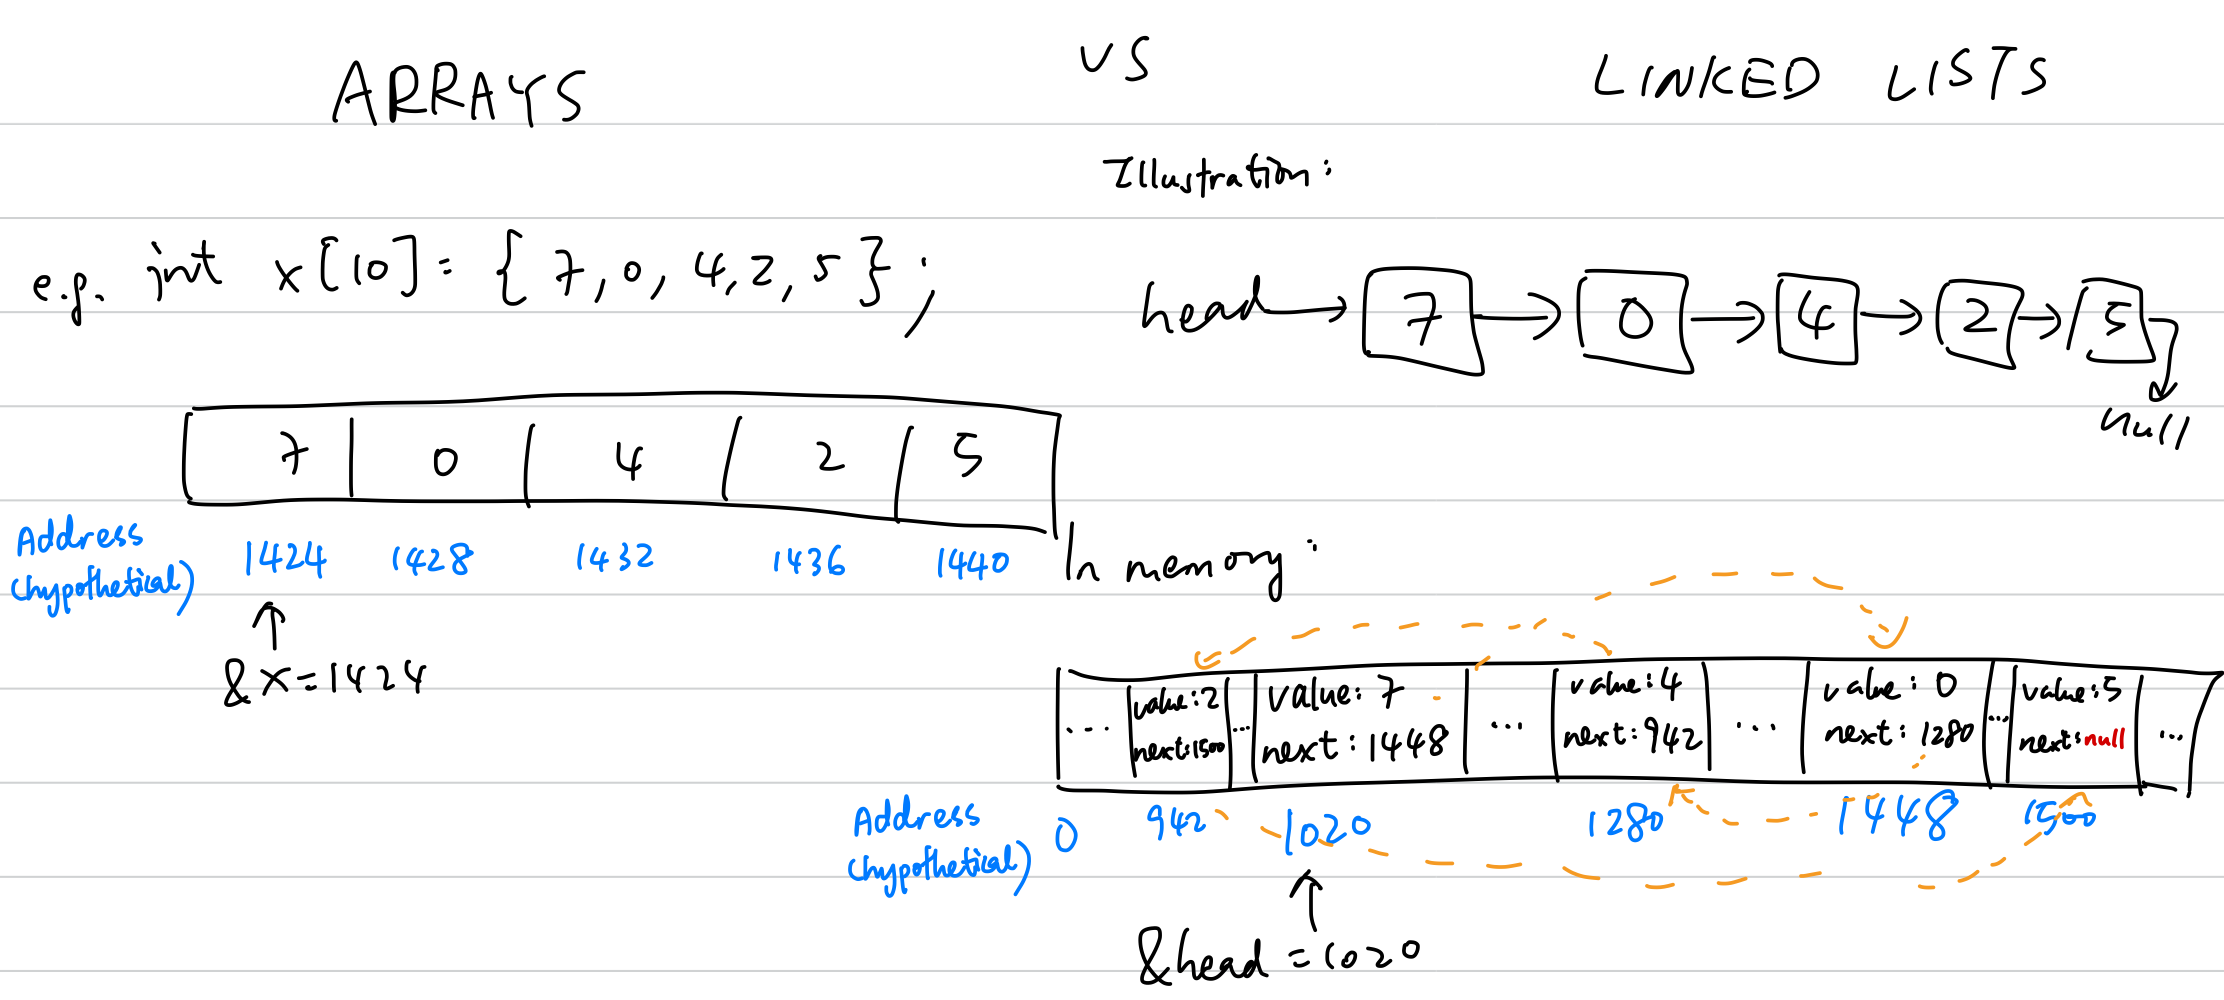
\includegraphics[width=15cm]{ch5-linkedlist1}

\subsection{Contrasting linked lists and arrays}

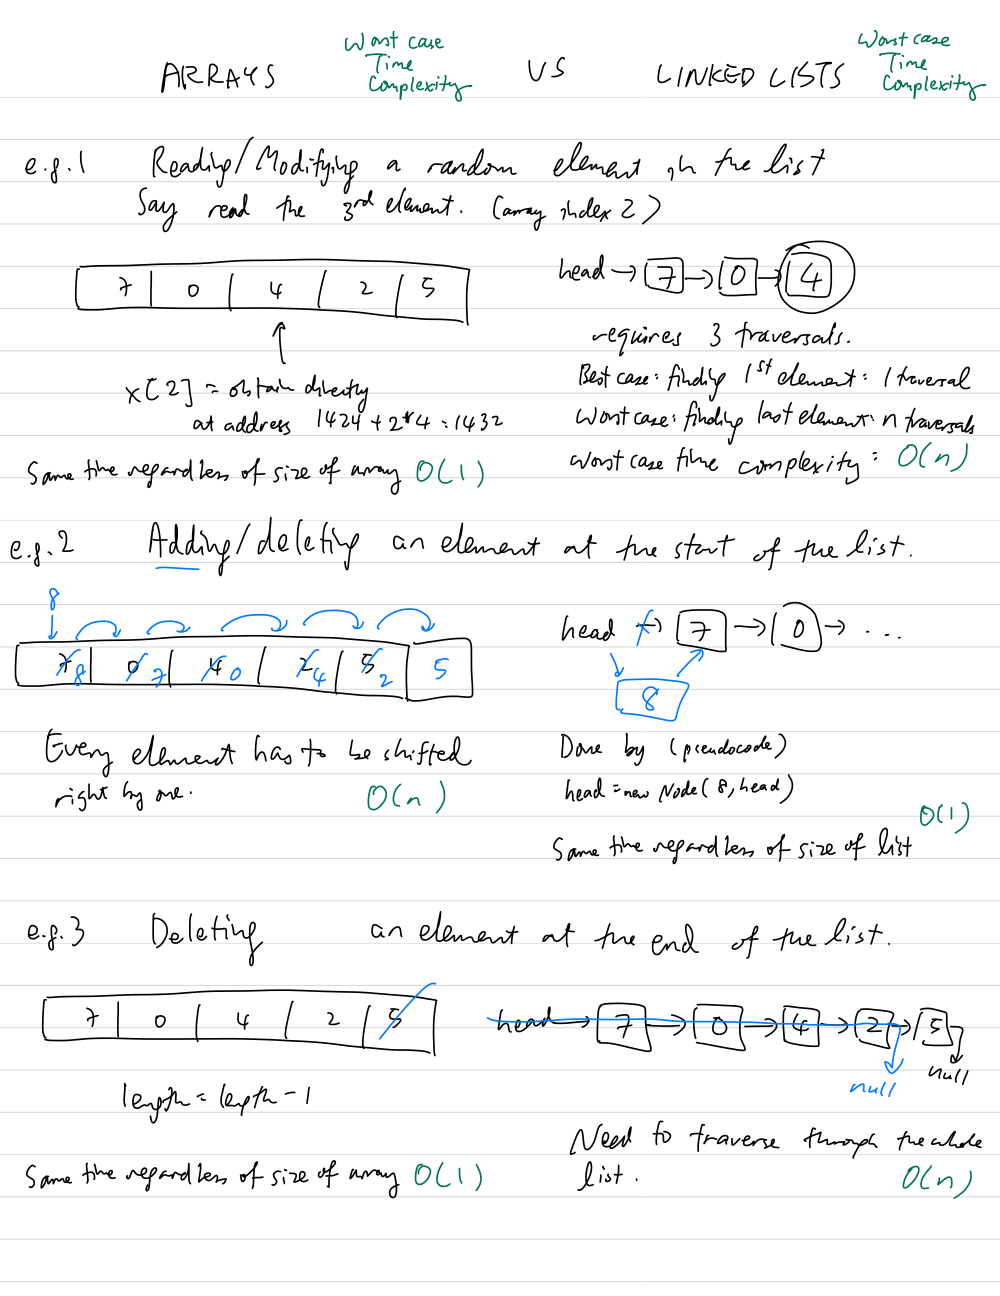
\includegraphics[width=15cm]{ch5-linkedlist2}

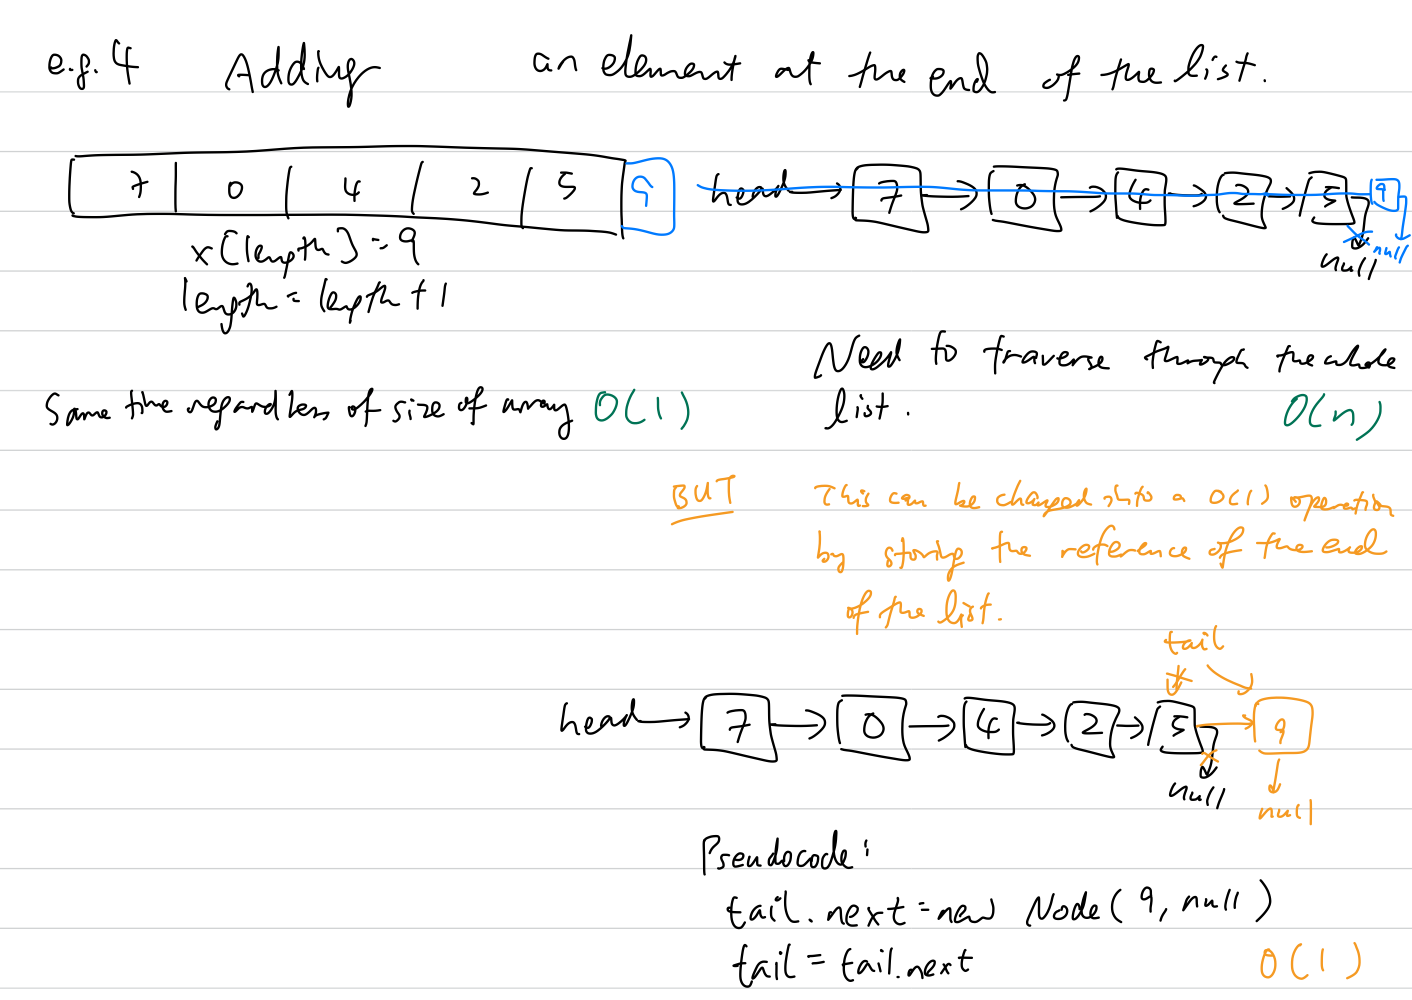
\includegraphics[width=15cm]{ch5-linkedlist3}

\section{Time complexity}

You may noticed the weird symbols in green in the above table. This is what we call the \textbf{big-O notation}\index{big-O notation}. It is used to describe time complexity\index{time complexity}, that is how computational work needed scales as the problem scales in size. Work is usually measured in terms of number of copies, traversals, or comparisons, depending on what our aim actually is. Size is usually measured in terms of size of the array/ linked list.\footnote{There is a very rigorous mathematical definition to the big-O notation, but it is not required in understanding what it is.}

Some processes above have a time complexity of $O(1)$, that means the same amount of work is required no matter how long the array/ linked list is. This is fantastic news! 

While some other processes have a time complexity of $O(n)$, that means we have to do more work as the array/linked list lengthens, this is still manageable. 

Some other processes you will encounter in the next few chapters have a time complexity of $O(n^2)$, this is bad news, because the amount of work would quickly go out of hand as n grows.

You will also encounter $\log$\footnote{The logarithm function: $b^c = a$ then $log_b a = c$, where $b$ is the base} in the big-O notation. Don't be afraid, it is good news, because $\log n$ scales slower than n. When we describe big-O notation the log base can be ignored.

We will usually analyze the worst case time complexity, as we want to know about the weaknesses of the algorithms.\footnote{Out of scope: The best case time complexity is usually not meaningful, and it is difficult to analyze the average case time complexity because it is difficult to define 'average'}

\section{Conclusion}
As you can see, linked lists and arrays have different efficiencies when performing different operations. There is no 'better' data structure, it is the job of we computer scientists to figure out which data structure should be used based on the scenario. Both linked lists and arrays can be used to implement stacks and queues and the algorithms that I will mention in the coming chapters. 

Yet I do not advise you to code using linked lists in C++, in fact I will not do so in this piece of notes, because it is quite troublesome\footnote{Out of scope: It is possible in C++, as it includes some Object Oriented Programming (OOP) features, but without automatic garbage collecting and a large boilerplate for OOP, there are better languages to implement linked lists, like Java, Scala, or Python.
}.
